\documentclass[UTF8, a4paper]{ctexart}
\usepackage{listings}
\usepackage{xcolor}
\usepackage{fontenc}
\usepackage{amsmath}
\usepackage{mathptmx}
\usepackage{subcaption}
\usepackage[hmargin=1.25in,vmargin=1in]{geometry}
\usepackage{stix}
\usepackage[colorlinks=true]{hyperref}
\usepackage{fontspec}
\usepackage{xeCJK}
\usepackage{ruby}
\usepackage{graphicx}
\usepackage{fancyhdr} 
\usepackage{float}

\setmainfont{Times New Roman}
\setmonofont{Consolas}
\setCJKmonofont{华文仿宋}
\graphicspath{{figure/}}
\CTEXsetup[format={\Large\bfseries}]{section}
\pagestyle{fancy}
\lhead{}
\chead{}
\rhead{}
\renewcommand{\headrulewidth}{0pt}
\title{《泡泡堂》大作业设计报告}
\author{2016011108 孙天宇}
\lstset
{
    breaklines=true,
    tabsize=3,
    showstringspaces=false
}
\lstdefinestyle{Common}
{
    extendedchars=\true,
    language={[Visual]Basic},
    frame=single,
    %===========================================================
    framesep=3pt,%expand outward.
    framerule=0.4pt,%expand outward.
    xleftmargin=3.4pt,%make the frame fits in the text area. 
    xrightmargin=3.4pt,%make the frame fits in the text area.
    %=========================================================== 
    rulecolor=\color{red}
}

\lstdefinestyle{A}
{
    style=Common,
    backgroundcolor=\color{yellow!10},
    %basicstyle=\scriptsize\color{black}\ttfamily,
    basicstyle=\small\color{black}\ttfamily,
    keywordstyle=\color{orange},
    identifierstyle=\color{cyan},
    stringstyle=\color{red},
    commentstyle=\color{black}
}
\hypersetup{linktoc=all, plainpages=false, hidelinks, urlcolor=blue}

\begin{document}
\maketitle
\section{游戏设置}
此次游戏画布大小设置为1200$ \times $900,通常笔记本电脑的分辨率为1920$\times$ 1080,而缩放与布局往往不是100\%,
因此可能会导致游戏画面不能完全显示(或失真模糊),因此首先需要修改电脑显示设置图\ref{fig:gameSetup}(a)所示:将更改文本、应用等项目的大
小设置为100\%。
  \begin{figure}[h]
    \centering
    \subcaptionbox{电脑显示分辨率设置\label{fig:subfig1}}
        {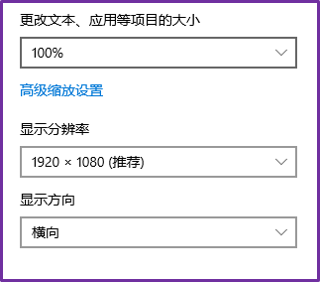
\includegraphics[width=0.45\textwidth]{setup.png}}
    \hspace{0.05\textwidth}
    \subcaptionbox{游戏界面大小\label{fig:subfig2}}
        {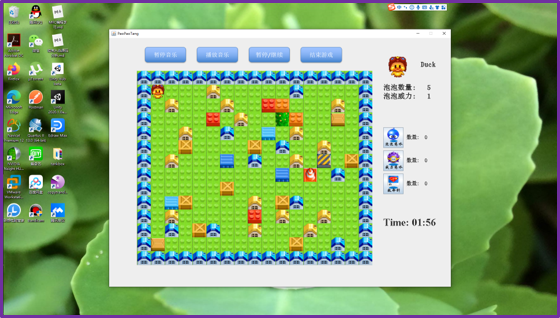
\includegraphics[width=0.45\textwidth]{ui.png}}
    \caption{游戏设置}
    \label{fig:gameSetup}
  \end{figure}

\section{基础功能与说明}
本次大作业实现采用了MVC模式,将整个游戏分为模型、视图、控制器三个部分。代码结构如下所示。整个流程是从主函数开始,首先加载gui
中的界面,然后资源加载器加载资源文件,游戏控制器加载地图等组件。当点击开始游戏,游戏线程启动,每隔20ms刷新各个游戏元素的状态。
\begin{lstlisting}[style=A]
config/         包含了游戏的配置文件,如图片路径、道具属性、地图信息等  
controller/     包含了游戏控制器与游戏组件的控制器
gui/            包含了游戏开始界面、游戏界面与结束界面
main/           程序入口
model/          游戏中的元素实体类,地板、箱子、泡泡、道具、人物等
resourceloader/ 资源加载器,从config文件夹中读取游戏的配置信息  
thread/         各种线程,如背景音乐、游戏刷新、键盘监听线程等。 
\end{lstlisting}
\subsection{游戏基本功能}
实现了开始游戏,结束游戏,暂停/继续游戏。玩家在游戏过程中可以随时暂停/继续/结束游戏。
游戏的状态控制实现在conttroller.GameController类中,其设置了running字段记录游戏运行状态。
当玩家暂停游戏时,键盘监听线程不再接收玩家的键盘输入,游戏线程停止刷新游戏组件状态,实现了游戏暂停的效果。
  \begin{figure}[H] % use float package if you want it here
    \centering
    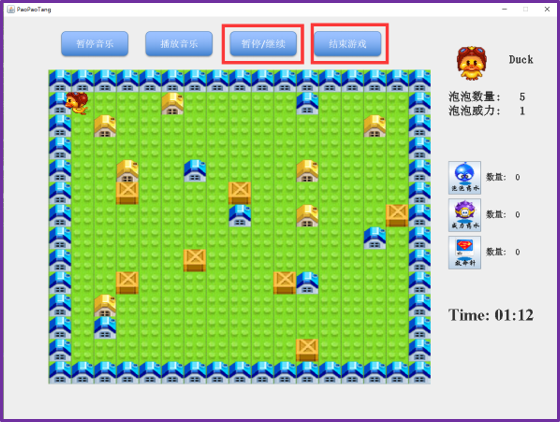
\includegraphics[width=0.80\textwidth]{control.png}
    \caption{基本游戏功能}
    \label{fig:basic}
  \end{figure}
\subsection{游戏生成与规则}
实现了游戏地图、箱子、障碍物与人物的生成,生成地图采用读取相关的地图配置文件。

游戏规则,实现了人物控制,游戏中可以通过W/A/S/D或上/下/左/右键来控制人物的移动,当人物遇到障碍物时,无法移动。
实现了空格键放置泡泡,泡泡爆炸范围受到障碍物等影响。泡泡威力可以增加。以上规则实现情况如下图所示
  \begin{figure}[h]
    \centering
    \subcaptionbox{人物遇障碍物停止\label{fig:subfig1}}
        {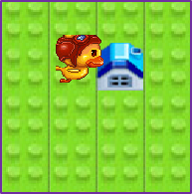
\includegraphics[width=0.23\textwidth]{move.png}}
    \hspace{0.01\textwidth}
    \subcaptionbox{放置泡泡\label{fig:subfig2}}
        {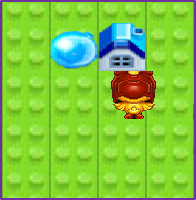
\includegraphics[width=0.23\textwidth]{plantbomb.png}}
    \hspace{0.01\textwidth}
    \subcaptionbox{泡泡爆炸(3s后)\label{fig:subfig2}}
        {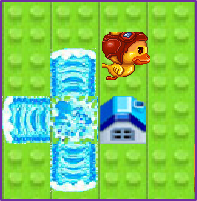
\includegraphics[width=0.23\textwidth]{explode1.png}}
    \hspace{0.01\textwidth}
    \subcaptionbox{泡泡威力增加\label{fig:subfig2}}
        {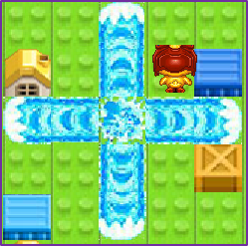
\includegraphics[width=0.23\textwidth]{power.png}}
    \caption{游戏规则实现}
    \label{fig:gameSetup}
  \end{figure}

泡泡爆炸冲击箱子后,箱子会消失,并依概率随机产生游戏道具泡泡药水(0.5)、威力药水(0.3)、救命针(0.2)。
玩家可以走到位置,拾取道具。可以通过鼠标点击来使用道具,泡泡爆炸具有连锁反应。玩家受到冲击后会处于濒死状态,
此时只能使用救命针,速度降为原1/4。
\begin{figure}[h]
    \centering
    \subcaptionbox{箱子破碎后生成道具\label{fig:subfig1}}
        {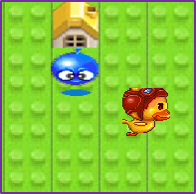
\includegraphics[width=0.23\textwidth]{gameprops.png}}
    \hspace{0.01\textwidth}
    \subcaptionbox{鼠标点击使用道具\label{fig:subfig2}}
        {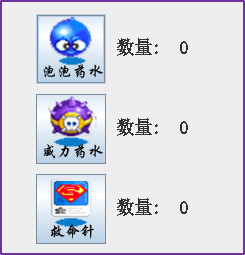
\includegraphics[width=0.23\textwidth]{userprops.png}}
    \hspace{0.01\textwidth}
    \subcaptionbox{连环爆炸\label{fig:subfig2}}
        {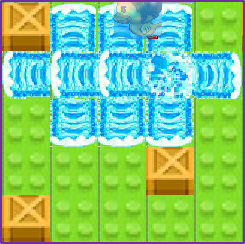
\includegraphics[width=0.23\textwidth]{serialbomb.png}}
    \hspace{0.01\textwidth}
    \subcaptionbox{人物濒死状态\label{fig:subfig2}}
        {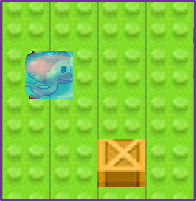
\includegraphics[width=0.23\textwidth]{dying.png}}
    \caption{游戏规则实现}
    \label{fig:gameSetup}
  \end{figure}

 代码设计,对于地图中的每一种元素都继承了superObject父类,每个实体都有碰撞判断,状态刷新,图片显示等接口。在ObjectController类中
 采用Map维护每一种地图元素的列表。游戏线程(GameThread)每隔20ms刷新一次所有地图元素的状态, 并进行爆炸与箱子碰撞判断、人物与道具碰撞判断,
 人物与爆炸碰撞判断、爆炸与泡泡连锁爆炸判断、游戏结果判断。


 \subsection{难度选择}
 在游戏开始界面可以进行地图的选择,总共包含了三种地图,分别对应初级模式、中级模式、高级模式。点击相关按钮可以进入到不同的
 地图环境中。
\begin{figure}[h]
    \centering
    \subcaptionbox{选择地图\label{fig:subfig1}}
        {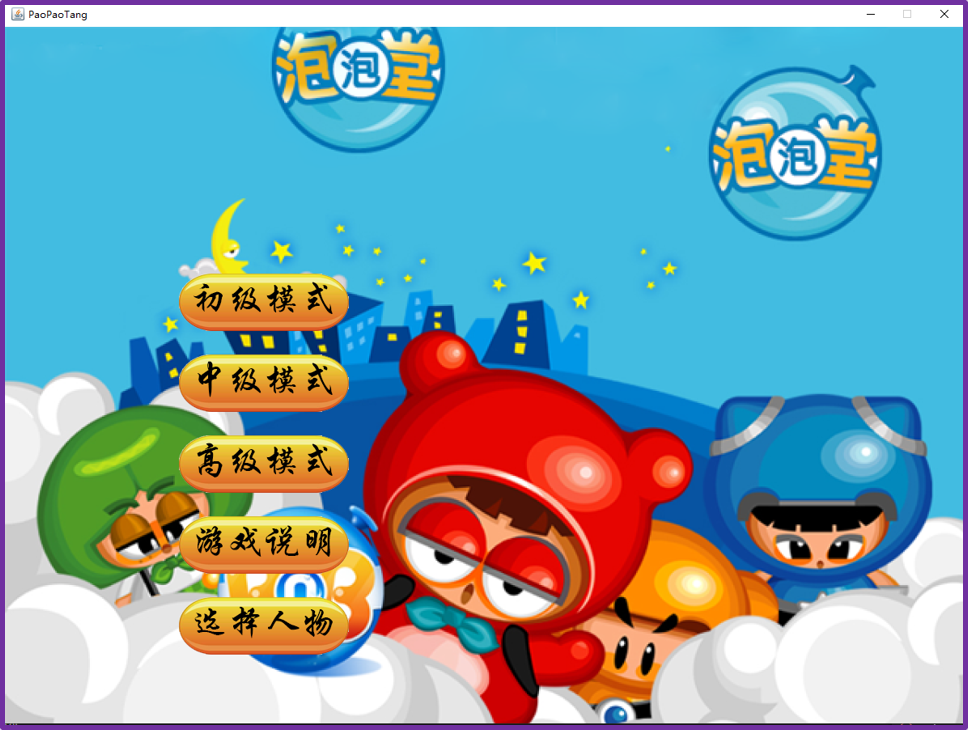
\includegraphics[width=0.23\textwidth]{start.png}}
    \hspace{0.01\textwidth}
    \subcaptionbox{初级模式\label{fig:subfig2}}
        {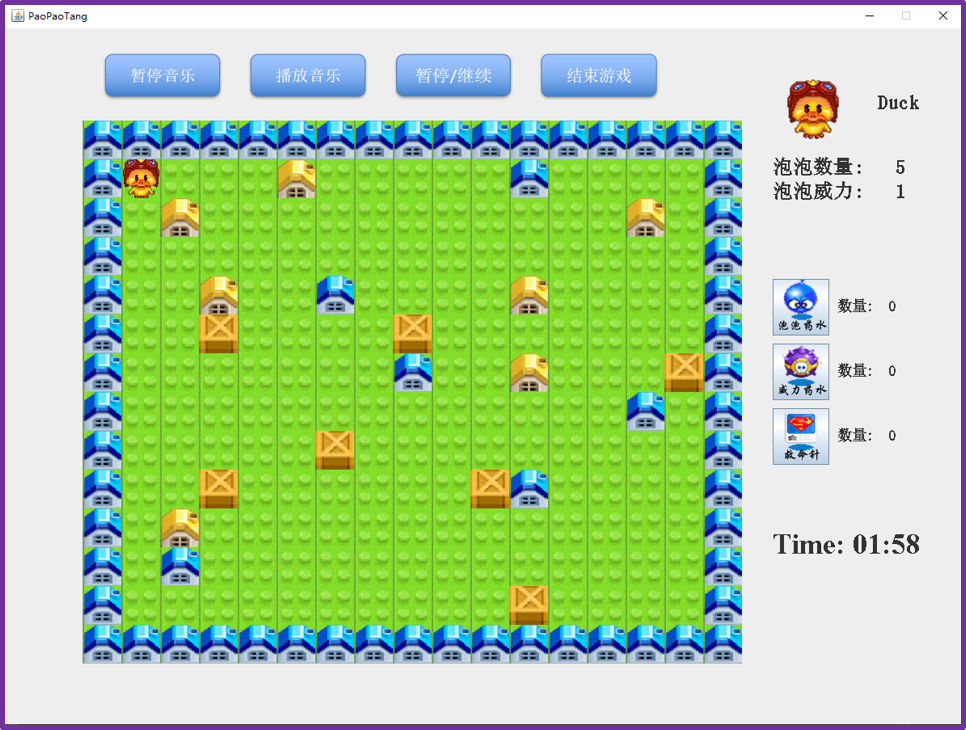
\includegraphics[width=0.23\textwidth]{primary.png}}
    \hspace{0.01\textwidth}
    \subcaptionbox{中级模式\label{fig:subfig2}}
        {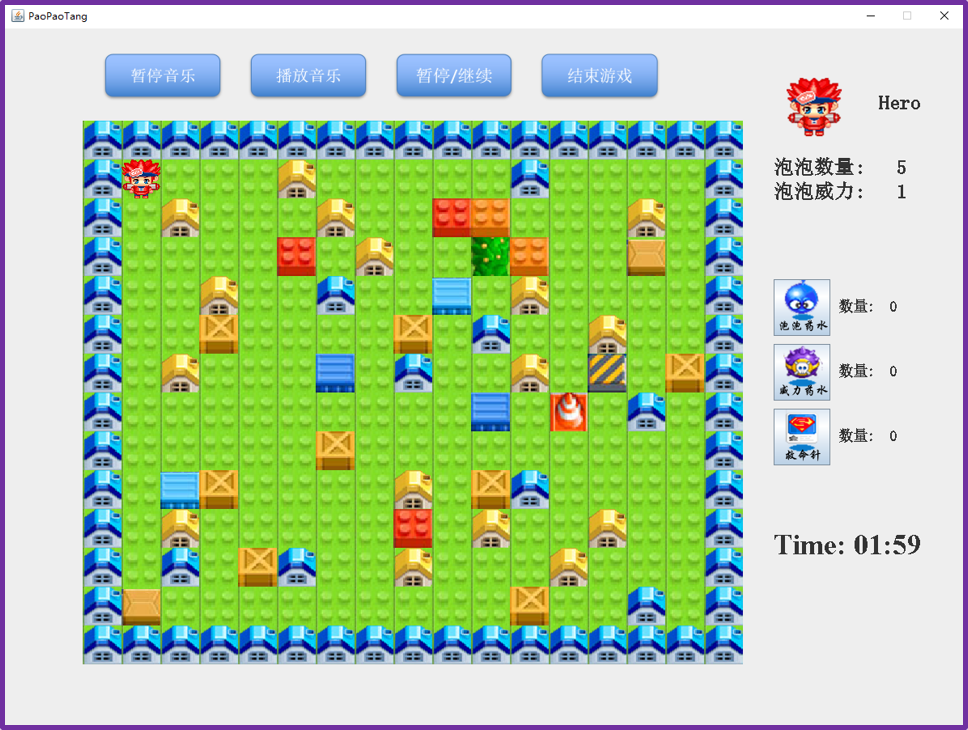
\includegraphics[width=0.23\textwidth]{middle.png}}
    \hspace{0.01\textwidth}
    \subcaptionbox{高级模式\label{fig:subfig2}}
        {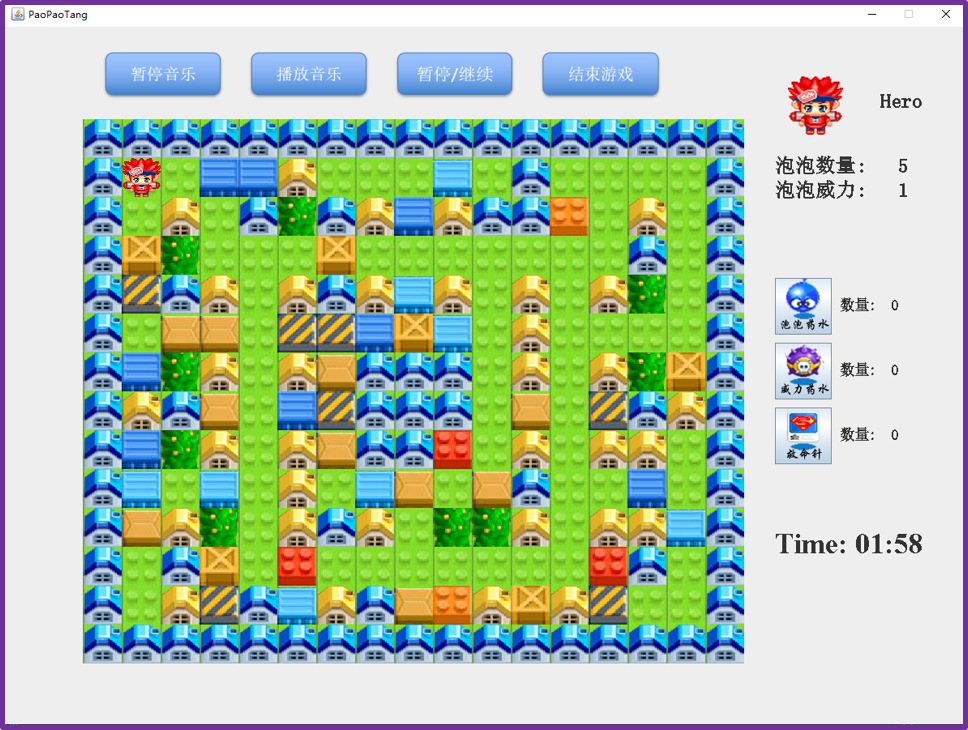
\includegraphics[width=0.23\textwidth]{advanced.png}}
    \caption{游戏难度选择}
    \label{fig:gameSetup}
  \end{figure}

\subsection{用户交互}
用户可以使用键盘A/W/S/D与↑/↓/←/→来控制人物的移动方向。可以使用SPACE空格键,放置泡泡。 

可以使用鼠标点击道具栏中的道具来使用泡泡药水、威力药水、救命针道具。

\subsection{界面美观度}
游戏状态栏,显示时间信息与玩家信息。
道具栏,玩家可以通过鼠标点击来使用道具。
  \begin{figure}[h]
    \centering
    \subcaptionbox{游戏状态栏\label{fig:subfig1}}
        {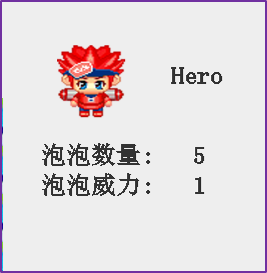
\includegraphics[width=0.45\textwidth]{playerinfo.png}}
    \hspace{0.05\textwidth}
    \subcaptionbox{道具栏与时间\label{fig:subfig2}}
        {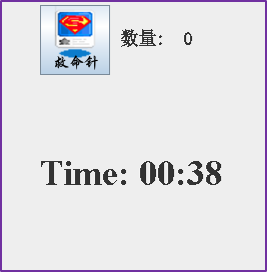
\includegraphics[width=0.45\textwidth]{time.png}}
    \caption{状态栏与道具栏}
    \label{fig:gameSetup}
  \end{figure}
   \begin{figure}[h]
    \centering
    \subcaptionbox{游戏胜利界面\label{fig:subfig1}}
        {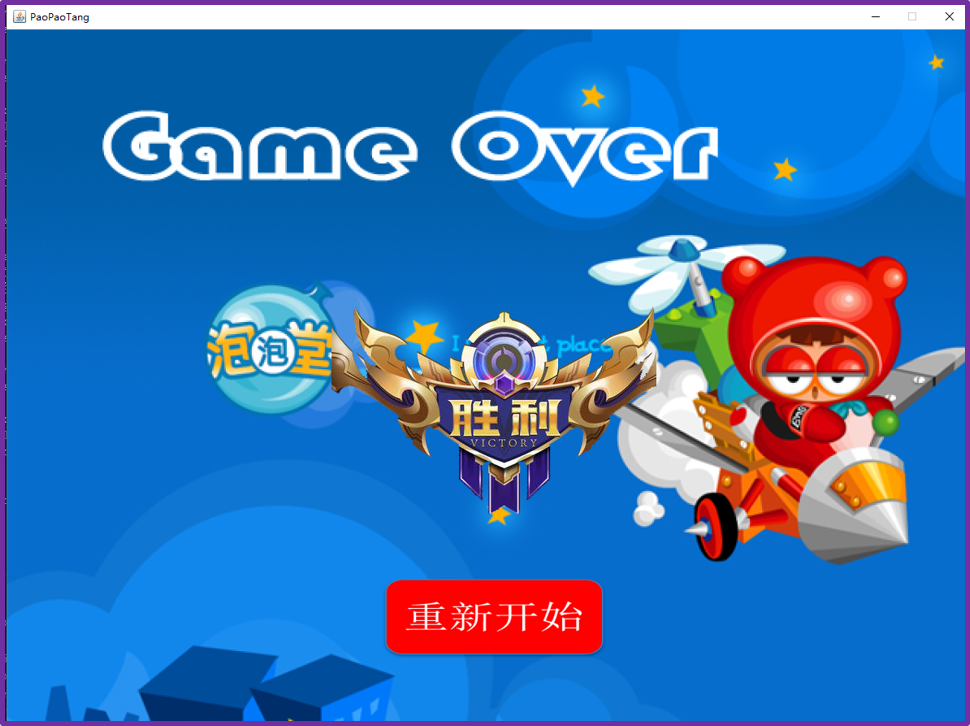
\includegraphics[width=0.45\textwidth]{victory.png}}
    \hspace{0.05\textwidth}
    \subcaptionbox{游戏失败界面\label{fig:subfig2}}
        {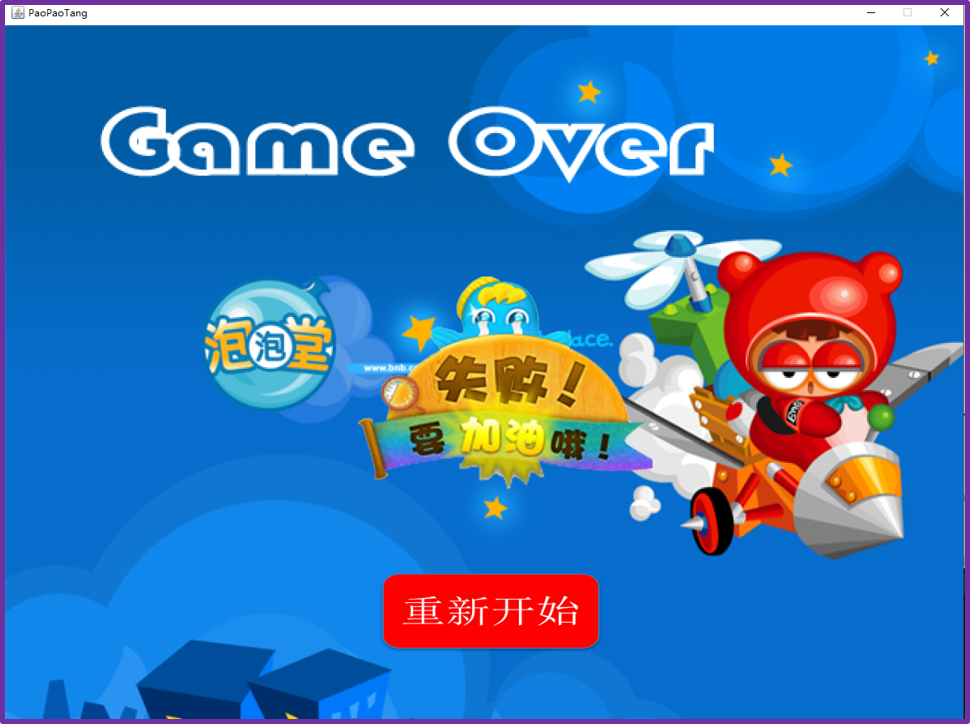
\includegraphics[width=0.45\textwidth]{failure.png}}
    \caption{胜利与失败界面}
    \label{fig:gameSetup}
  \end{figure}
\section{提高功能}
\subsection{游戏动画}
实现了人物移动,泡泡冲击,角色濒死等动画效果。
\subsection{游戏音效}
实现了背景音乐,并可以通过按钮来控制播放/暂停音乐,当进入游戏时自动播放背景音乐,游戏结束后自动停止播放。
 \begin{figure}[H] % use float package if you want it here
    \centering
    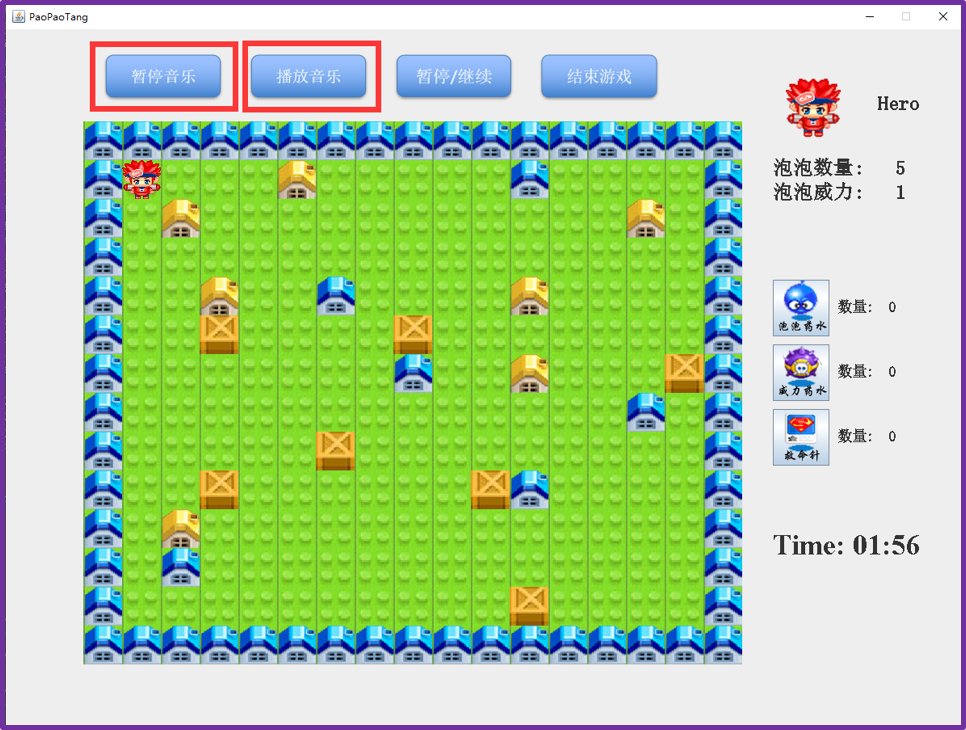
\includegraphics[width=0.80\textwidth]{playmusic.png}
    \caption{游戏背景音乐播放与暂停}
    \label{fig:music}
  \end{figure}
\subsection{换装}
可以通过开始界面来选择人物,总共有两个人物可供选择。  
 \begin{figure}[H] % use float package if you want it here
    \centering
    
\includegraphics[width=0.80\textwidth]{change.png}
    \caption{选择人物}
    \label{fig:select}
  \end{figure}
\end{document}
